% Add `ngerman` to documentclass for German docs
\documentclass[12pt, a4paper]{article}
\usepackage{a4wide}
\usepackage{setspace}
\usepackage[utf8]{inputenc}

\usepackage{url}
\usepackage[hidelinks]{hyperref}
\usepackage{minted}
\usemintedstyle{trac}

% inline code
\newcommand{\code}[1]{\texttt{#1}}

% Uncomment for German
%\usepackage[ngerman]{babel}

% For generating template dummy text
\usepackage{lipsum}

\usepackage{myColors}
\usepackage{myFooter}
\usepackage{myTitle}
\project{CS 432 Web Science}
\author{Derek Goddeau}
\title{Assignment One}
\supervisor{Michael L. Nelson}

\doublespace
\pagestyle{hacker}

\begin{document}
\maketitle

\newpage

\section{POST to a from with \code{curl}}

In order to submit \code{POST} data to a form using \code{curl} first
it must be ensured that the form accepts \code{POST} data. This can be
done by viewing the page source and verifying that the form tag has
\code{method="post"} as in the \href{https://nostarch.com}{nostarch.com}
search bar form tag shown somewhat abridged below.

\begin{minted}{html}

<form action="/" method="post" id="search-theme-form">
<input name="search_theme_form" value="" class="form-text"/>
<input name="op" value="Search" class="form-submit"/>
<input type="hidden" name="form_build_id" value="form-6Skwd"/>
<input type="hidden" name="form_id" value="search_theme_form"/>
</form>
\end{minted}

\noindent
In order to
craft the \code{curl} command the \code{-d} flag can be used along
with the \code{"name=value"} pattern for each input to the form
where \code{name} is copied from each input tag and \code{value}
is changed in the fields where the default values are not desired.

%%%%%%%%%%%%%%%%%%%%%
% Curl command used %
%%%%%%%%%%%%%%%%%%%%%
\begin{minipage}{\linewidth} % prevent splitting between pages
\vspace{2em}
\begin{minted}{bash}

curl -L -i -o results.html \
           -d "search_theme_form=$1" \
           -d "op=Search" \
           -d "form_build_id=form-6SkwdjCka872mUDOLyJspWzIHtkBGso7f5RMZ2fGr9U" \
           -d "form_id=search_theme_form" \
           https://www.nostarch.com/
\end{minted}
\vspace{2em}
\end{minipage}

\noindent
The command \code{curl\_post.sh car} will return
a page with the search results for "car" on \href{https://nostarch.com}
{nostarch.com}. Inspecting the output \code{results.html} the
\code{HTTP/1.1 200 OK} after a single redirect and lack of a 405
Method not allowed error means the request was successful.

%%%%%%%%%%%%%%%%%%%%%%%%%%%
% curl results screenshot %
%%%%%%%%%%%%%%%%%%%%%%%%%%%
\href{https://gitlab.com/datenstrom/cs532-s17/blob/master/assignments/assignment_one/curl/results.html}{
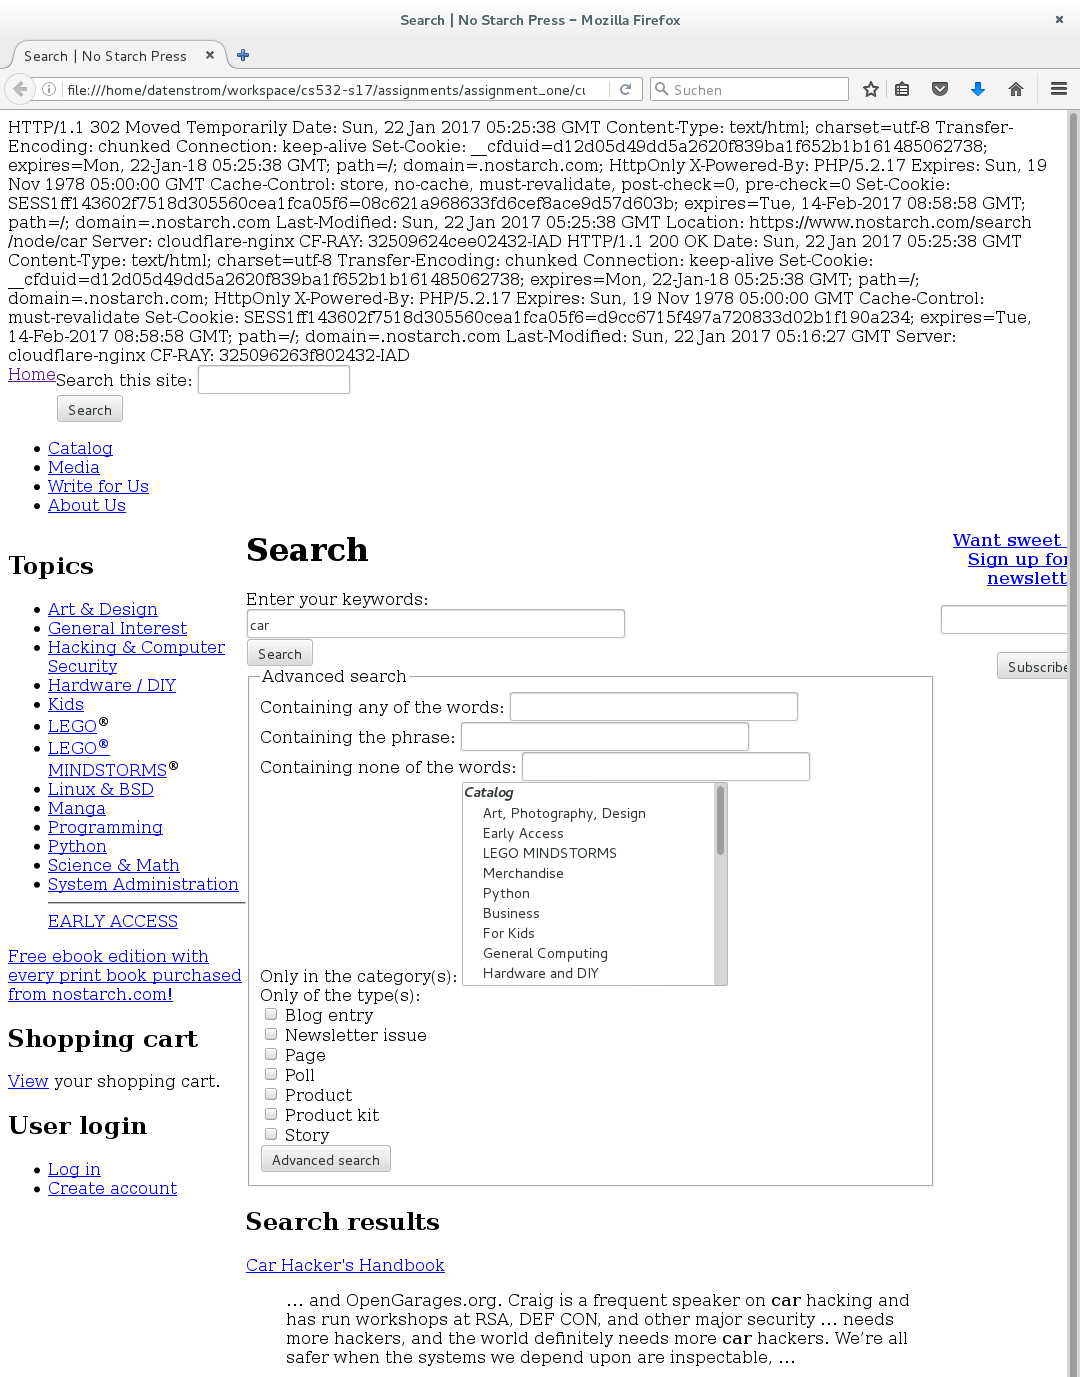
\includegraphics[width=\textwidth]{dia/curl_screenshot.png}
}



%                          Pyton                                      %
%%%%%%%%%%%%%%%%%%%%%%%%%%%%%%%%%%%%%%%%%%%%%%%%%%%%%%%%%%%%%%%%%%%%%%%
\section{A Python program that finds PDFs}

The \href{https://gitlab.com/datenstrom/cs532-s17/tree/master/assignments/assignment_one/common_house_spider}
{\code{Common House Spider}} can take any number of URIs as input
optionaly from a specified file with the \code{-f} flag, and use
multiple threads using the \code{-t} flag.
It outputs all PDF URIs on the page and the PDF size as reported
by the server. Note that the \code{-u} or \code{--ugly} parameter must be
passed to print first and last URI.

\vspace{2em}
\begin{minted}[fontsize=\scriptsize]{bash}
datenstrom@redacted$ python cli.py -t 2 www.nostarch.com/carhacking https://www.nostarch.com/blackhatpython -u
[*] Crawling pages:
www.nostarch.com/carhacking
https://www.nostarch.com/blackhatpython
[*] Spinning up with 2 threads
[*] Thread 1 discovered 3 PDF links for https://www.nostarch.com/blackhatpython
[*] Thread 1 removed 0 duplicate PDF files

First link: http://www.nostarch.com/download/BlackHatPython_ch07.pdf
Last link: https://www.nostarch.com/download/BlackHatPython_ch07.pdf
PDF size: 88339

First link: http://www.nostarch.com/download/BlackHatPython_dTOC.pdf
Last link: https://www.nostarch.com/download/BlackHatPython_dTOC.pdf
PDF size: 54377

First link: http://www.nostarch.com/download/BlackHatPython_Index.pdf
Last link: https://www.nostarch.com/download/BlackHatPython_Index.pdf
PDF size: 116530

[*] Thread 0 discovered 5 PDF links for www.nostarch.com/carhacking
[*] Thread 0 removed 1 duplicate PDF file

First link: http://www.nostarch.com/download/Car Hackers Handbook_sample_Chapter5.pdf
Last link: https://www.nostarch.com/download/Car%20Hackers%20Handbook_sample_Chapter5.pdf
PDF size: 1713557

First link: http://www.nostarch.com/download/Car Hackers Handbook_sample_Chapter5.pdf
Last link: https://www.nostarch.com/download/Car%20Hackers%20Handbook_sample_Chapter5.pdf
PDF size: 1713557

First link: http://www.nostarch.com/download/Car Hackers Handbook_sample_dTOC.pdf
Last link: https://www.nostarch.com/download/Car%20Hackers%20Handbook_sample_dTOC.pdf
PDF size: 594880

First link: http://www.nostarch.com/download/Car Hackers Handbook_sample_index.pdf
Last link: https://www.nostarch.com/download/Car%20Hackers%20Handbook_sample_index.pdf
PDF size: 660045

First link: https://www.usenix.org/system/files/login/articles/login_summer16_19_books.pdf
Last link: https://www.usenix.org/system/files/login/articles/login_summer16_19_books.pdf
PDF size: 81289

[*] PDF links discovered in 20.1669859409 seconds
\end{minted}
\vspace{1em}


%%%%%%%%%%%%%%%%
% Required URI %
%%%%%%%%%%%%%%%%
It is also both Python 2.6+ and Python 3 compatible:

\vspace{1em}
\begin{minted}[fontsize=\scriptsize]{bash}

datenstrom@redacted$ python3 cli.py http://www.cs.odu.edu/~mln/teaching/cs532-s17/test/pdfs.html -u
[*] Crawling pages:
http://www.cs.odu.edu/~mln/teaching/cs532-s17/test/pdfs.html
[*] Spinning up with 1 thread
[*] Thread 0 discovered 11 PDF links for http://www.cs.odu.edu/~mln/teaching/cs532-s17/test/pdfs.html
[*] Thread 0 removed 0 duplicate PDF files

[*] Thread 0 discovered 11 PDF links for http://www.cs.odu.edu/~mln/teaching/cs532-s17/test/pdfs.html
[*] Thread 0 removed 0 duplicate PDF files

First link: http://www.cs.odu.edu/~mln/pubs/ht-2015/hypertext-2015-temporal-violations.pdf
Last link: http://www.cs.odu.edu/~mln/pubs/ht-2015/hypertext-2015-temporal-violations.pdf
PDF size: 2184076

First link: http://www.cs.odu.edu/~mln/pubs/tpdl-2015/tpdl-2015-annotations.pdf
Last link: http://www.cs.odu.edu/~mln/pubs/tpdl-2015/tpdl-2015-annotations.pdf
PDF size: 622981

First link: http://arxiv.org/pdf/1512.06195
Last link: https://arxiv.org/pdf/1512.06195.pdf
PDF size: 1748961

First link: http://www.cs.odu.edu/~mln/pubs/tpdl-2015/tpdl-2015-off-topic.pdf
Last link: http://www.cs.odu.edu/~mln/pubs/tpdl-2015/tpdl-2015-off-topic.pdf
PDF size: 4308768

First link: http://www.cs.odu.edu/~mln/pubs/tpdl-2015/tpdl-2015-stories.pdf
Last link: http://www.cs.odu.edu/~mln/pubs/tpdl-2015/tpdl-2015-stories.pdf
PDF size: 1274604

First link: http://www.cs.odu.edu/~mln/pubs/tpdl-2015/tpdl-2015-profiling.pdf
Last link: http://www.cs.odu.edu/~mln/pubs/tpdl-2015/tpdl-2015-profiling.pdf
PDF size: 639001

First link: http://www.cs.odu.edu/~mln/pubs/jcdl-2014/jcdl-2014-brunelle-damage.pdf
Last link: http://www.cs.odu.edu/~mln/pubs/jcdl-2014/jcdl-2014-brunelle-damage.pdf
PDF size: 2205546

First link: http://bit.ly/1ZDatNK
Last link: http://www.cs.odu.edu/~mln/pubs/jcdl-2015/jcdl-2015-temporal-intention.pdf
PDF size: 720476

First link: http://www.cs.odu.edu/~mln/pubs/jcdl-2015/jcdl-2015-mink.pdf
Last link: http://www.cs.odu.edu/~mln/pubs/jcdl-2015/jcdl-2015-mink.pdf
PDF size: 1254605

First link: http://www.cs.odu.edu/~mln/pubs/jcdl-2015/jcdl-2015-arabic-sites.pdf
Last link: http://www.cs.odu.edu/~mln/pubs/jcdl-2015/jcdl-2015-arabic-sites.pdf
PDF size: 709420

First link: http://www.cs.odu.edu/~mln/pubs/jcdl-2015/jcdl-2015-dictionary.pdf
Last link: http://www.cs.odu.edu/~mln/pubs/jcdl-2015/jcdl-2015-dictionary.pdf
PDF size: 2350603

[*] PDF links discovered in 14.306671047210693 seconds

\end{minted}
\vspace{2em}

\newpage
\section{Graph Structure}

The sample graph below is the dataset that will be used to demonstrate the
\code{SCC}, \code{IN}, \code{OUT}, \code{DISCONNECTED}, \code{TUBES}, and
\code{TENDRILS} components. The heatmaping in figure one is based on the
degree for each node. Using this directed graph the single \code{SCC}
component can be found, it contains all of the nodes which are reachable
from eachother. In this sample graph these nodes are \code{A},
\code{B}, \code{C}, and \code{G} which are color coded red in figure 2.

Once the \code{SCC} has been discovered, the \code{IN} and \code{OUT} components
can be found. These consist of the nodes that link only into or out of the
\code{SCC} respectively. The \code{IN} component consists of nodes
\code{O}, \code{M}, and \code{P} which are colored green in figure 2.
The \code{OUT} components are \code{H} and \code{D}, yellow in figure 2.

\begin{figure}[h]
    \centering
    \caption{Graph heatmap by node degree}
    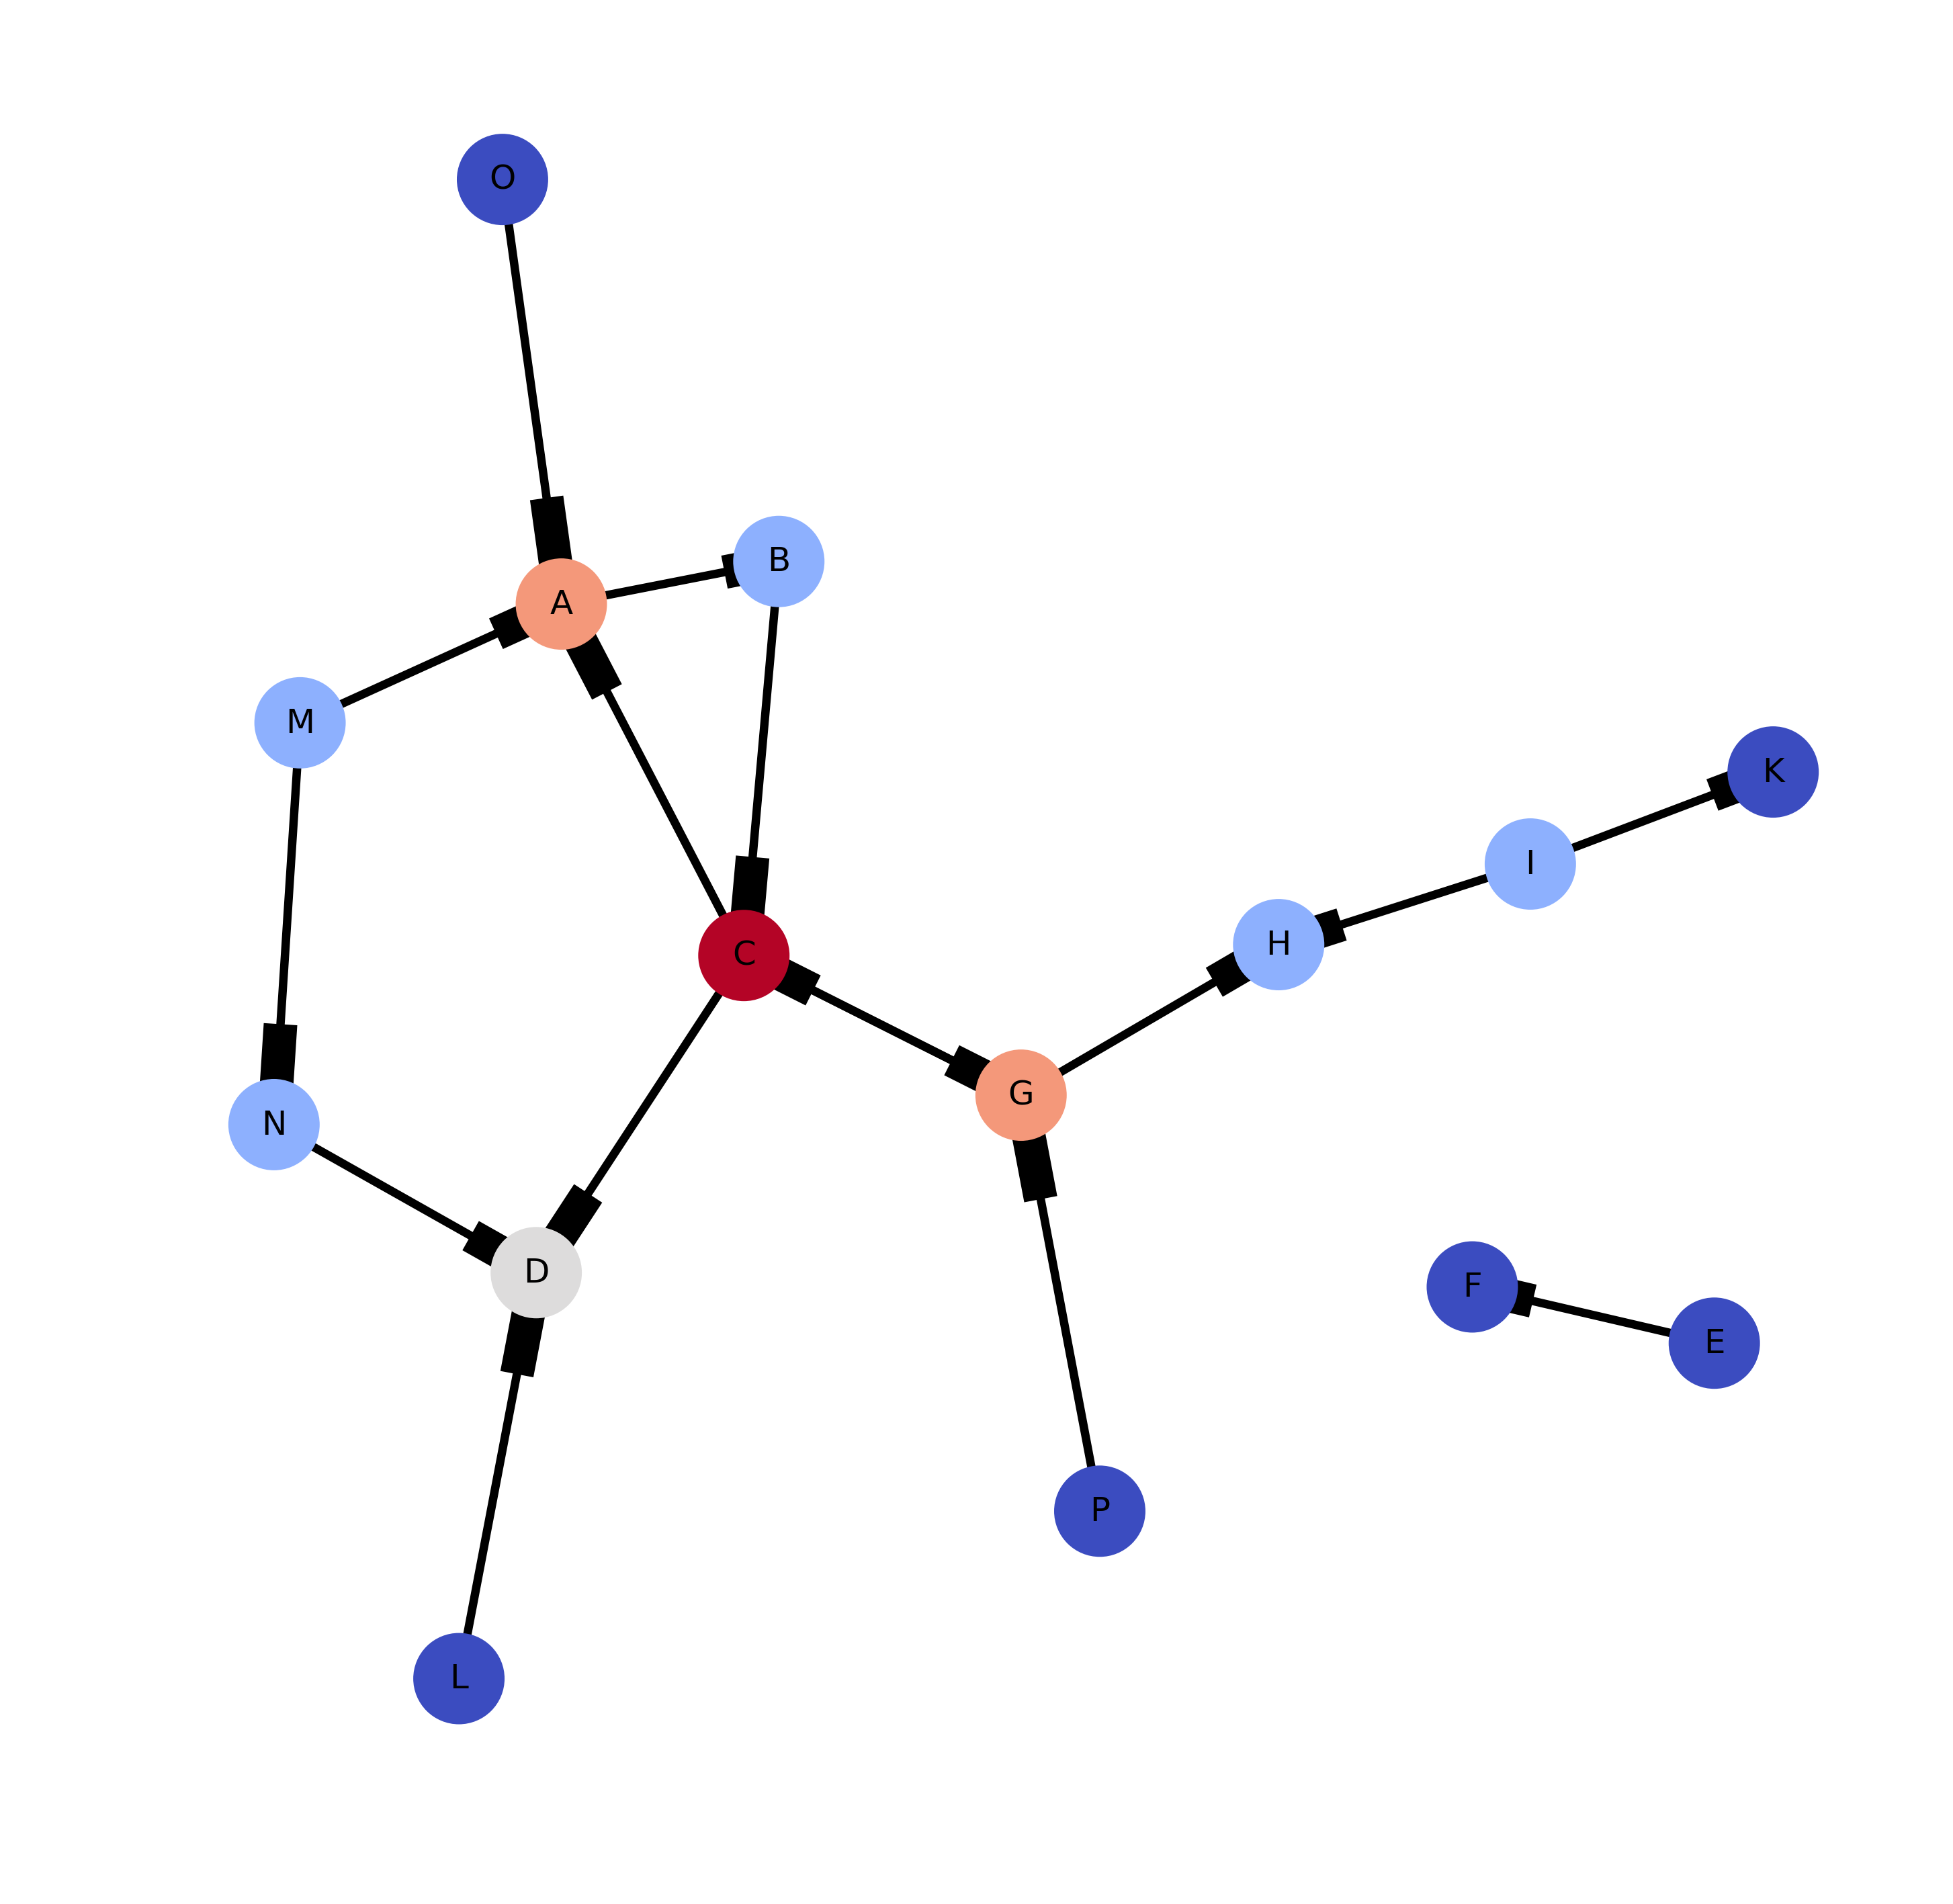
\includegraphics[width=0.70\textwidth]{dia/graph_heatmap.png}
\end{figure}

\newpage
The \code{DISCONNECTED} component contains all nodes unreachable from
the other components, which are the grey nodes \code{F} and \code{E}.
\code{TUBES} are nodes which connect \code{IN} and \code{OUT} nodes,
there is only one node in this example \code{N} colored purple.
Finally the \code{TENDRILS} are the blue nodes \code{I}, \code{K},
and \code{L} which shoot off of the \code{IN} and \code{OUT}
components but do not directly interact with the \code{SCC}.

\begin{table}[h]
    \centering
    \begin{tabular}{|c|c|c|}
        \hline
        Component    & Color  & Nodes \\ \hline
        SCC          & red    & 4     \\ \hline
        IN           & green  & 3     \\ \hline
        OUT          & yellow & 2     \\ \hline
        TENDRILS     & blue   & 3     \\ \hline
        TUBES        & purple & 1     \\ \hline
        DISCONNECTED & grey   & 2     \\ \hline
    \end{tabular}
\end{table}

\begin{figure}[h]
    \centering
    \caption{Graph components}
    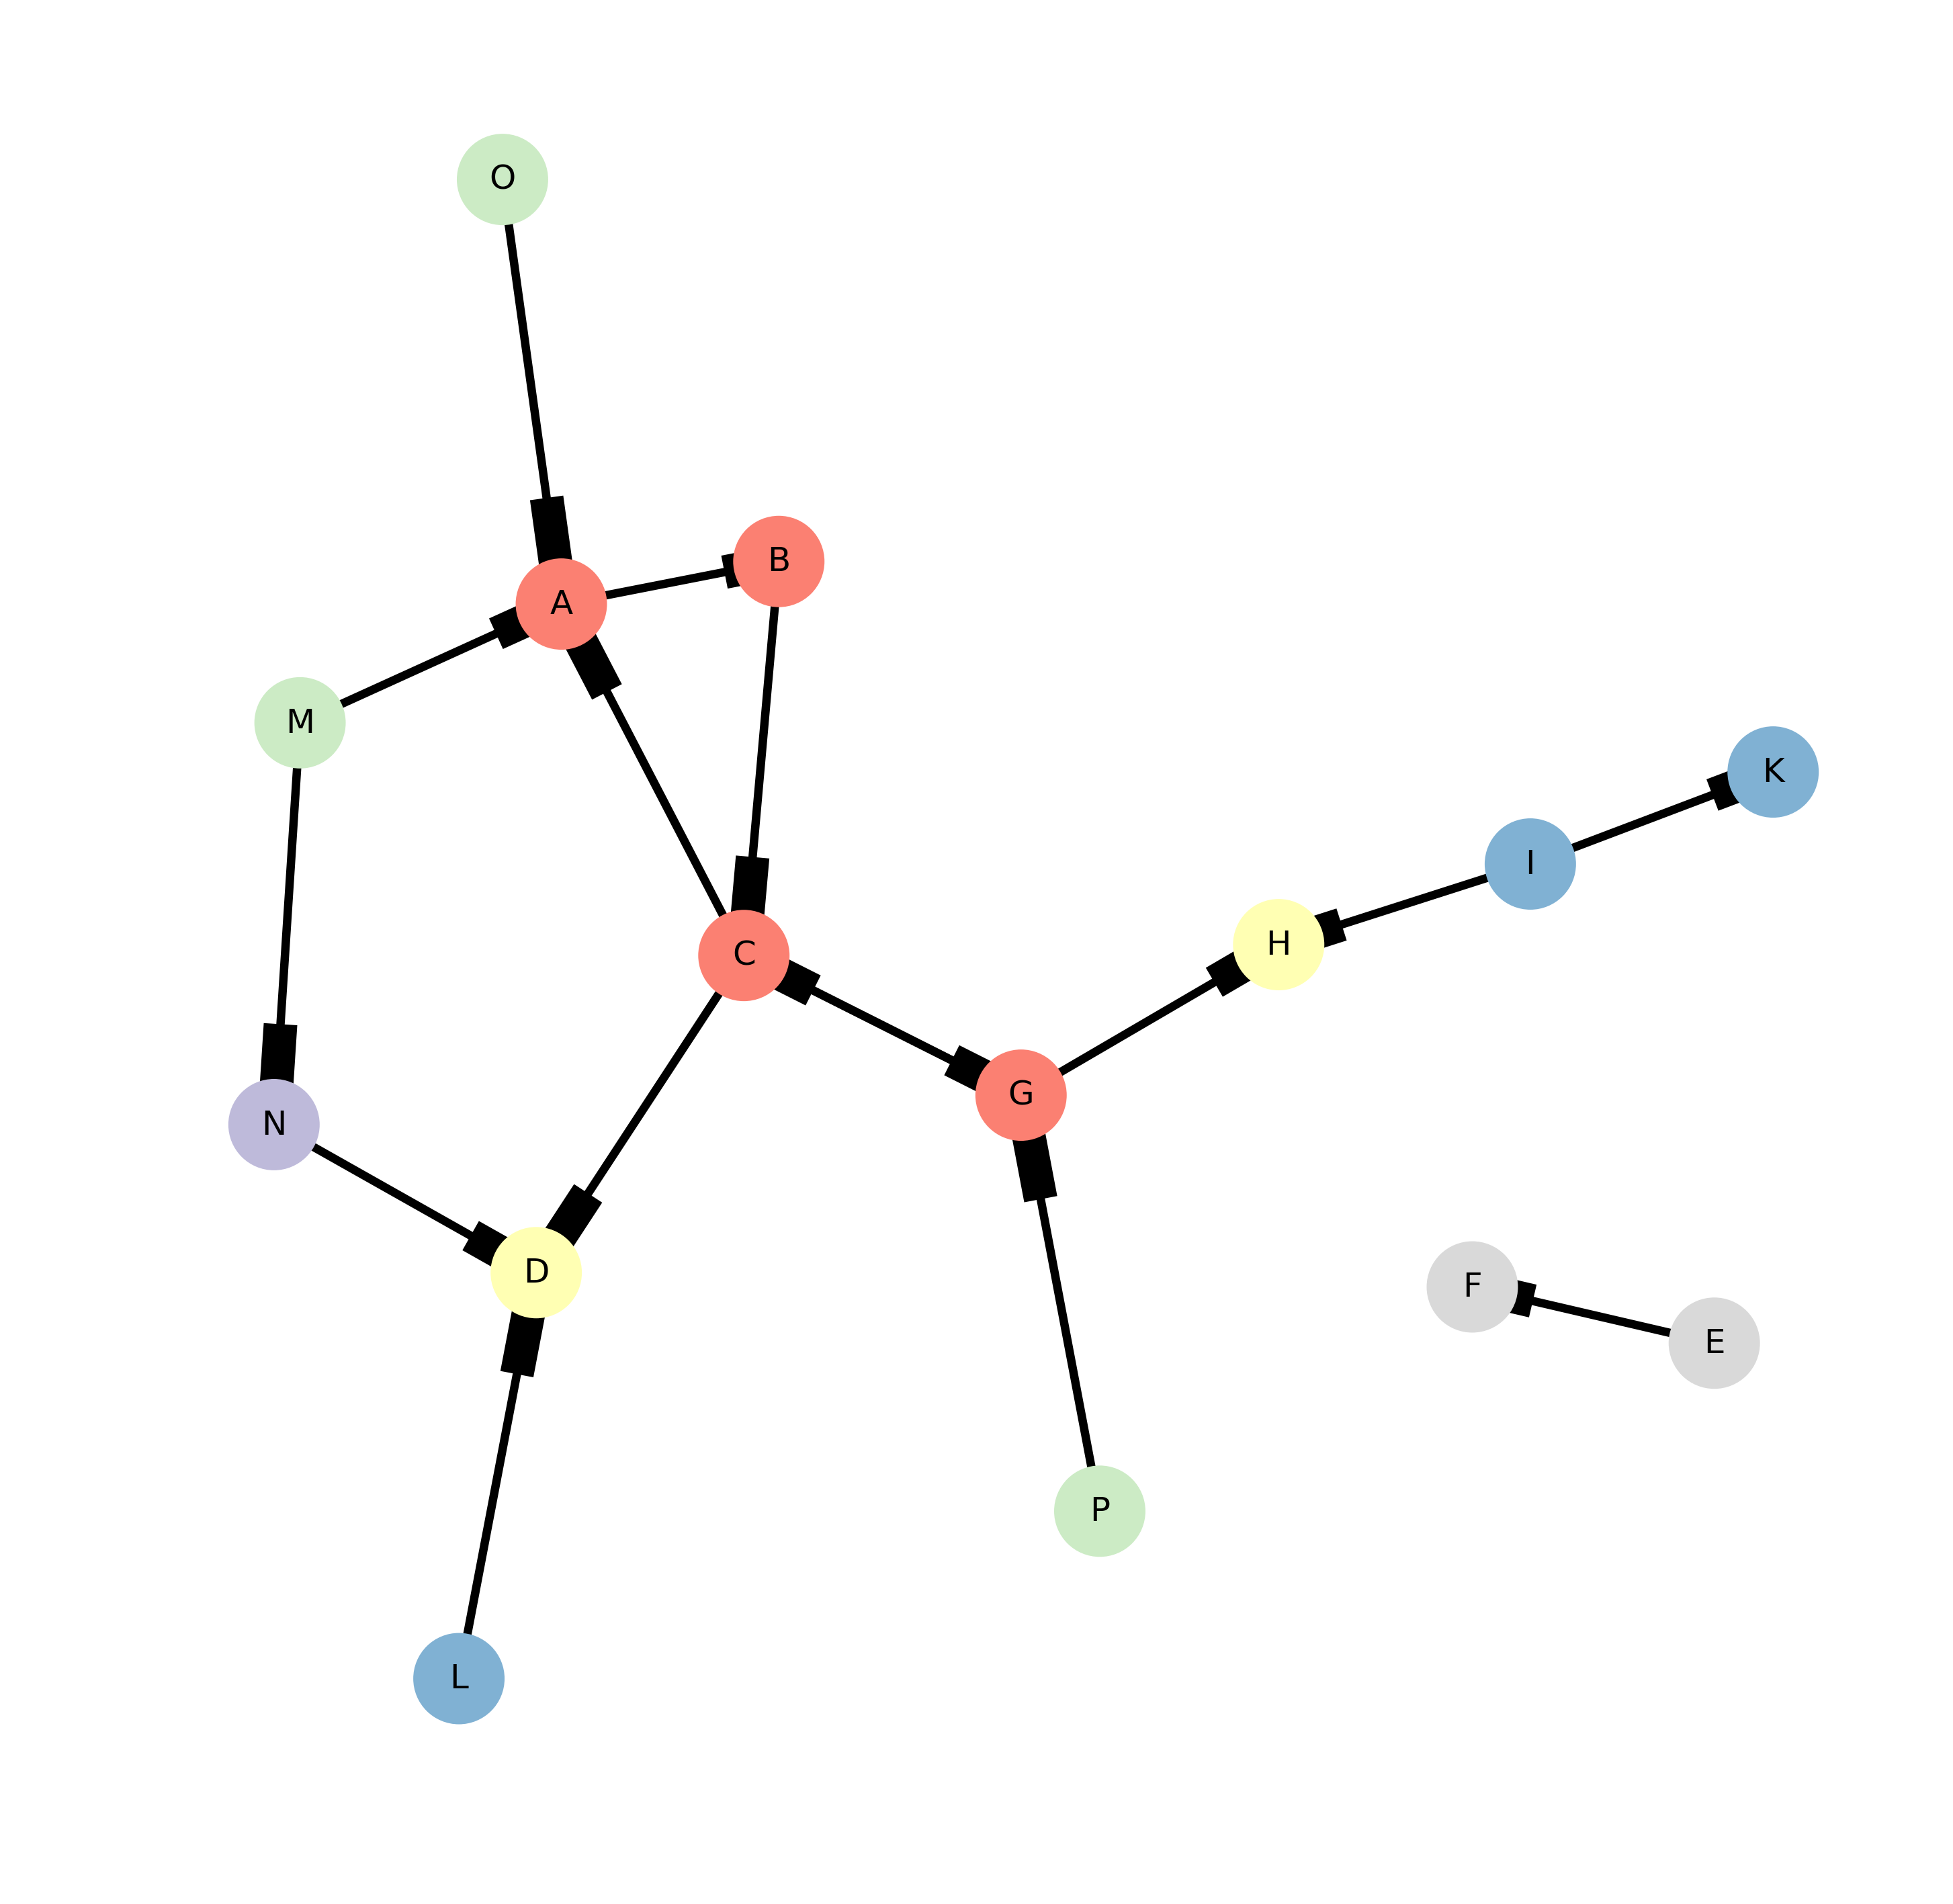
\includegraphics[width=0.70\textwidth]{dia/graph_components.png}
\end{figure}


\end{document}
